% !TeX TS-program = pdflatex
% !BIB TS-program = bibtex
\documentclass{article}
% links
\usepackage[
  colorlinks,
  citecolor=magenta,
]{hyperref}
\newcommand{\hreftt}[1]{\href{#1}{\texttt{#1}}}
% references
\usepackage[
  style=numeric,
  doi=false,
  url=false,
  isbn=false,
  natbib=true,
  backend=bibtex,
  sorting=none,
]{biblatex}
\addbibresource{A.bib}
\addbibresource{main.bib}
% floats
\usepackage{booktabs,multicol,subcaption,rotating,graphicx}
\newcommand{\tn}[1]{{\textsuperscript{~#1}}}
\newcommand{\tnt}[2][]{\textsuperscript{#1~}{#2}}
\newcommand{\floatfoot}[2][\linewidth]{\vskip 1ex
  \begin{minipage}{#1}\footnotesize#2\end{minipage}}
\graphicspath{
  {fig/}
  {fig/app/}
}
% temp
\usepackage{xspace}
\newcommand{\x}[1]{\input{/home/jesse/phd/proj/sr/out/tex/#1}\unskip}
\newcommand{\xd}[1]{\x{#1.q2}~[\x{#1.q1},~\x{#1.q3}]\xspace}
\newcommand{\xdm}[1]{\x{#1.q2}~[\x{#1.q0},~(\x{#1.q1},~\x{#1.q3}),~\x{#1.q4}]\xspace}
\newcommand{\xdmdef}{median [min,~(IQR),~max]\xspace}
\newcommand{\tx}[1]{\textit{t\textsubscript{#1}}}
% appendix stuff
\usepackage{float,tikz}
\usepackage[mode=text,group-separator={,}]{siunitx}
\newcommand{\searchsize}{\footnotesize}
\newcommand{\searchstyle}{\ttfamily\searchsize}
\newcommand{\st}[1]{{\searchstyle#1}}
\newcommand{\tabitem}{{\textbullet}~~}
\newcommand{\onecol}{{\let\clearpage\relax\onecolumn}}
\newcommand{\twocol}{{\let\clearpage\relax\twocolumn}}
\newcommand{\pseudocite}[1]{%
  \parbox{0.5\linewidth}{%
    \parbox{6ex}{\hfill\parencite{#1}}
    \parbox{6ex}{\centering\citeyear{#1}}
    \citeauthor{#1}%
}}
\newlength{\tsep}\setlength{\tsep}{1ex}
\newcommand{\itab}[2]{%
  \x{api/#1/#2.q2} & ( \x{api/#1/#2.q1}, \x{api/#1/#2.q3} ) & \x{api/#1/n.#2}}
\newcommand{\xtab}[1]{\itab{inc}{#1} & & \itab{chi}{#1} & }
\newcommand{\ptab}[2]{\itab{inc}{#1} & \x{api/inc/#2.pval} & \itab{chi}{#1} & \x{api/chi/#2.pval}}
\usepackage{pdfpages}
\newcommand{\includepdfcmd}[2]{%
  \includepdf[pages=1, width=\textwidth,pagecommand={#2}]{#1}%
  \includepdf[pages=2-,width=\textwidth,pagecommand={}]{#1}%
}
\def\countrylist{Angola, Benin, Botswana, Burkina Faso, Burundi, Cameroon, Cape Verde, Central African Republic, Chad, Comoros, Democratic Republic of the Congo, Djibouti, Equatorial Guinea, Eritrea, eSwatini, Ethiopia, The Gabon, Gambia, Ghana, Guinea, Guinea-Bissau, Côte d'Ivoire, Kenya, Lesotho, Liberia, Madagascar, Malawi, Mali, Mauritania, Mauritius, Mozambique, Namibia, Niger, Nigeria, Republic of the Congo, Reunion, Rwanda, Sao Tome and Principe, Senegal, Seychelles, Sierra Leone, Somalia, South Africa, South Sudan, Sudan, Tanzania, Togo, Uganda, Zambia, Zimbabwe}
\def\bibidB{Salomon2005,Abbas2006,Granich2009,Hallett2009b,Bacaer2010,Pretorius2010,Metzger2011,Yusuf2012,Andrews2012,Granich2012,Wagner2012,Abbas2013,Long2013,Cremin2013,Alsallaq2013,Nichols2014,Nichols2014a,Alistar2014,Eaton2014a,Ying2015,Low2015,Khademi2015,Gilbert2015,Heaton2015,Rahman2016,Gilbert2016,Blaizot2016,Ying2016,Barnighausen2016,Heffernan2016,Maheu-Giroux2017a,Maheu-Giroux2017,Volz2017,Blaizot2017,Mukandavire2018,Guillon2018,Akudibillah2018,Stuart2018,deMontigny2018,Hauser2019}
\def\bibidAxB{Johnson2006,Baggaley2006,Wilson2006,Bacaer2008,Chigidi2009,Williams2010,Nyabadza2011,Barnighausen2012,Wagner2013,Decker2013,Wirtz2013,Shafer2014,Hove-Musekwa2014,Braithwaite2014,Nichols2014b,Abu-Raddad2014,Anderson2014,Alistar2014a,Cori2014,Stover2014,Wirtz2014,Korenromp2015,Knight2015,Kerr2015,Fraser2015,Kassa2015,Bekker2015,Shannon2015,Blaizot2015,Smith2016,Atun2016,Shattock2016,McGillen2016,Johnson2016,Sharma2016,Akudibillah2017,Alsallaq2017,Anderson2017,Chiu2017,Johnson2017b,Stuart2017,McGillen2017,Cremin2017,Ross2018,Anderson2018,Anderson2018a,Omondi2018,Woods2018,Stevens2018,Stopard2019,Beacroft2019a,Reidy2019,Omondi2019,Maheu-Giroux2019}
\def\plotlistdist{
  api.prev.cat/HIV prevalence at $t_0$ (\%),
  api.prev/HIV prevalence at $t_0$ (\%),
  api.inc/HIV incidence at $t_0$ (per 1000 PY),
  api.phase/HIV epidemic phase,
  hiv.n/Number of HIV states,
  art.rbeta/Relative infectiousness on ART,
  act.n/Number of activity groups,
  age.n/Number of age groups,
  act.HRW.p/Proportion of women in the highest female activity group,
  act.HRM.p/Proportion of men in the client or highest activity male group
}
\def\plotlistapi{%
  api.prev/HIV prevalence at $t_0$ (\%),
  art.cd4/CD4 initiation criteria,
  api.phase/HIV epidemic phase,
  art.cov/ART intervention coverage target,
  art.rbeta/Relative infectiousness on ART
}
\usepackage{catchfile}
\newcommand{\filedef}[1]{\CatchFileDef\filedata{#1}{\endlinechar=-1}}
\refid{EPIDEMICS-D-21-00134}
\title{Risk heterogeneity in compartmental HIV transmission models of
  ART as prevention in Sub-Saharan Africa: A scoping review}
\author{Jesse~Knight, Rupert~Kaul, Sharmistha~Mishra}
\date{Dec 5, 2021}
%%%%%%%%%%%%%%%%%%%%%%%%%%%%%%%%%%%%%%%%%%%%%%%%%%%%%%%%%%%%%%%%%%%%%%%%%%%%%%%%
\begin{document}
%%%%%%%%%%%%%%%%%%%%%%%%%%%%%%%%%%%%%%%%%%%%%%%%%%%%%%%%%%%%%%%%%%%%%%%%%%%%%%%%
\maketitle
\tableofcontents
\clearpage
%\section*{Key Messages}\input{messages}
%\clearpage
% ==============================================================================
\section{Introduction} \label{s:intro}      Sub-Saharan Africa continues to bear the largest burden of HIV.  %SM: reviewed and rationale set up very nicely! no further edits :) 
As of 2019, two thirds (25.7 million) of all people living with HIV globally are in Sub-Saharan Africa, where
an estimated one million new HIV infections were acquired in 2019.\cite{AIDSinfo}
Data suggest that key populations, such as individuals engaged in sex work and men who have sex with men experience
disproportionate risks of HIV acquisition and onward transmission in Sub-Saharan Africa.
\cite{Baral2012,Beyrer2012,Mishra2012,Boily2015}
% SM: cite (data papers from reviews led by Baral; and also some modeling papers - see our tPAF paper we just did for published citations)
HIV treatment to reduce onward transmission remains a key element of combination HIV prevention.\cite{WHO2016ART}
Effective HIV treatment with antiretroviral therapy (ART) leads to viral load suppression
and has been shown to prevent HIV transmission between sex partners.\cite{Lundgren2015,Danel2015,Cohen2016}
\par
Following empirical evidence of partnership-level efficacy of ART
in preventing HIV,\cite{Lundgren2015,Danel2015,Cohen2016}
and model-based evidence of ``treatment as prevention'',\cite{Granich2009,Eaton2012,Cori2014}
several large-scale community-based trials of universal test-and-treat (UTT)
have recently been completed.\cite{Iwuji2018,Havlir2019,Hayes2019}
These trials found that over 2 to 4 years,
cumulative incidence under UTT did not significantly differ from
cumulative incidence under ART according to national guidelines.\cite{Havlir2019,Hayes2019,Iwuji2018}
Thus the population-level reductions in incidence anticipated from transmission modelling
were not observed in the trials.\cite{Baral2019,Havlir2020}
% SM: cite the transmission modeling statement
\par
One theme in the proposed explanations for limited population-level ART effectiveness
was heterogeneity in intervention coverage and its intersection with
heterogeneity in transmission risks.\cite{AbdoolKarim2019,Baral2019}
While viral suppression improved under UTT in all three trials,
21--54\% of study participants remained unsuppressed.\cite{Iwuji2018,Havlir2019,Hayes2019}
It has been suggested that populations experiencing barriers to viral suppression under UTT
may be at highest risk for onward transmission, including key populations like
female sex workers, men who have sex with men, and adolescent girls and young women.%
\cite{Hakim2018,Nyato2019,Green2020}
While widespread UTT scale-up may fill some of these coverage gaps,
equitable access to ART for marginalized populations remains an open challenge.
\par
Given the upstream and complementary role of transmission modelling
in estimating the impact of ART as prevention,\cite{Eaton2012,Delva2012},
% SM: but have not said anything about critical role of risk heterogenetiy yet to support the 'given' phrase in this statement,
%     so I think just introducing in the first paragraph, and then going directly into this statement here as edited flows
%     without us pre-editorializing (seeming like we are criticizing?)
we sought to critically appraise and examine the type and scope of risk heterogeneity captured
in mathematical models used to assess the prevention impacts of ART in Sub-Saharan Africa.
We conducted a scoping review with the following objectives.
Among dynamical compartmental models of sexual HIV transmission
that have been used to simulate the prevention impacts of ART in Sub-Saharan Africa:
\begin{enumerate}
\item\label{rq:1}
      In which epidemic contexts (geographies, populations, epidemic phases)
      have these models been applied?
\item\label{rq:2}
      How was the model structured to represent key factors of risk heterogeneity?
\item\label{rq:3}
      What are the potential influences of representations of risk heterogeneity
      on the projected prevention benefits of ART for all?
\end{enumerate}
\section{Methods}      \label{s:methods}    We conducted a scoping review according to the PRISMA extension for scoping reviews
(see Appendix~\ref{a:prisma} for checklist).
First, we developed a conceptual framework to organize
the assumptions and representations of risk heterogeneity
in compartmental HIV transmission models.
Then, we designed and implemented the search strategy,
and extracted the data relevant to the framework
to address the objectives.
% ==============================================================================
\subsection{Conceptual Framework for Risk Heterogeneity}
\label{ss:meth:framework}
For the review, we conceptualized ``factors of risk heterogeneity'', meaning
epidemiological stratifications and phenomena which may/not be included in transmission models.
Such factors include if/how populations, rates, and probabilities
are stratified along health, structural, and behavioural dimensions.
We defined the following 4 domains in which
different factors of risk heterogeneity might influence the transmission impact of ART.
\begin{itemize}
  \item \textbf{Biological Effects:}
  differential transmission risk within HIV disease course
  that coincides with differential ART coverage
  \cite{Pilcher2004}
  \item \textbf{Behaviour Change Effects:}
  differential transmission risk due to
  behavioural changes related to engagement in the ART cascade
  \cite{Ramachandran2016,Tiwari2020} % JK: TODO
  \item \textbf{Network Effects:}
  differential transmission risk within sub-populations
  that increase the challenge of epidemic control through core group dynamics
  \cite{Anderson1986,Boily1997,Watts2010,Dodd2010}
  \item \textbf{Coverage Effects:}
  differential transmission risk within sub-populations
  who also experience barriers to engaging in ART care and achieving viral suppression,
  such as youth and key populations
  \cite{Mountain2014,Lancaster2016,Hakim2018,Green2020}
\end{itemize}
We then compiled a list of key factors of risk heterogeneity,
and their possible mechanisms of influence on ART prevention impact (Table~\ref{tab:factors}).
\afterpage{%
  \newgeometry{margin=2cm}
  \begin{landscape}
    \captionof{table}{%
      Factors of heterogeneity in HIV transmission
      and their possible mechanisms of influence on the prevention impact of ART interventions}
    \footnotesize\centering
\begin{tabular}{llp{.35\linewidth}p{.4\linewidth}}
  \toprule
  \textbf{Factor}
& \textbf{MP\tn{a}}
& \textbf{Definition}
& \textbf{Possible mechanism(s) of influence on ART prevention impact}
\\
\midrule
  Acute Infection
& $\beta_i$
& Increased infectiousness immediately following infection \cite{Hollingsworth2008,Boily2009}
& \textbf{Biological}: transmissions during acute infection are unlikely to be prevented by ART
\\
  Late-Stage Infection
& $\beta_i$
& Increased infectiousness during late-stage infection \cite{Hollingsworth2008,Boily2009}
& \textbf{Biological}: transmissions during late-stage are more likely to be prevented by ART
\\
  Drug Resistance
& $\beta_i$
& Transmitted factor that requires regimen switch to achieve viral suppression \cite{DeWaal2018}
& \textbf{Biological}: transmissions during longer delay to achieving viral suppression will not be prevented by ART
\\
\midrule
  HIV Morbidity
& $c$; $\eta$
& Reduced sexual activity during late-stage disease \cite{Myer2010,McGrath2013}
& \textbf{Behaviour Change}: reduced morbidity via ART could increase HIV prevalence among the sexually active population
\\
  HIV Counselling
& $c$; $\eta$; $\kappa$
& Reduced sexual activity and/or increased condom use after HIV diagnosis \cite{Tiwari2020}
& \textbf{Behaviour Change}: increased HIV testing with ART scale up can contribute to prevention even before viral suppression is achieved
\\
\midrule
  Activity Groups
& $c$; $\kappa$
& Any stratification by rate of partnership formation \cite{Anderson1991}
& \textbf{Network}: higher transmission risk among higher activity
\\
  Age Groups
& $c$; $\kappa$
& Any stratification by age
& \textbf{Network \& Cascade}: higher transmission risk and barriers to viral suppression among youth \cite{Birdthistle2019,Green2020}
\\
  Key Populations
& $c$; $\kappa$
& Any epidemiologically defined higher risk groups \cite{WHO2016KP}
& \textbf{Network \& Cascade} higher transmission risk and barriers to viral suppression among key populations \cite{Hakim2018}
\\
  Group Turnover
& $\phi$
& Individuals move between activity groups and/or key populations reflecting sexual lifecourse \cite{Watts2010}
& \textbf{Network \& Cascade}: counteract effect of stratification due to shorter periods in higher risk \cite{Knight2020};
  viral suppression may be achieved only after periods of higher risk
\\
  Assortative Mixing
& $m$
& Any degree of assortative mixing (like-with-like) by age, activity, and/or key populations
& \textbf{Network}: assortative sexual networks compound effect of stratification \cite{Anderson1991}
\\
  Partnership Types
& $\eta$; $\kappa$
& Different partnership types are simulated, with different numbers of sex acts and/or condom usage \cite{Scorgie2012}
& \textbf{Network}: longer duration and lower condom use among main versus casual/sex work partnerships
  counteracts effect of stratification
\\
  ART Cascade Gaps
& $\tau$; $\alpha$
& Slower ART cascade transitions among higher activity groups or key populations \cite{Hakim2018,Green2020}
& \textbf{Cascade}: ART prevention benefits may be allocated differentially among risk groups
\\
\bottomrule
\end{tabular}
\floatfoot{\tnt[a]{MP: Model Parameters ---
  $\beta_i, \beta_s$: transmission probability per act (infectiousness, susceptibility);
$\eta$:      number of sex acts of each type per partnership;
$\kappa$:    proportion of sex acts unprotected by a condom;
$c$:         partnership formation rate;
$m$:         mixing matrix (probability of partnership formation);
$\mu$:       mortality rate;
$\nu$:       entry rate;
$\phi$:      internal turnover between activity groups;
$\tau$:      testing rate;
$\alpha$:    ART initiation rate (and retention-related factors).}
}

    \label{tab:factors}
  \end{landscape}
  \restoregeometry
\clearpage}
% ==============================================================================
\subsection{Search}
\label{ss:meth:search}
We searched MEDLINE and EMBASE via Ovid
using search terms related to Sub-Saharan Africa (SSA), HIV, and transmission modelling.
(Appendix~\ref{aa:search:terms}).
%did you use Covidence? if yes, include that in methods... (suggest checking Christine's paper re: some methods which might help and also read over other papers/guidelines on level of detail to include to ensure reproduciblity, etc?)
Duplicate studies were removed automatically %SM: how? (within Covidence?)
and also manually. %SM: how? did you check for duplicates manually?
Potentially relevant studies were identified by title and abstract screening, followed 
by full-text screening using the inclusion/exclusion criteria listed below. 
We then conducted data extraction from the full text and available supplementary material.
One reviewer (JK) conducted the search, screening, and data extraction.  
% ------------------------------------------------------------------------------
\subsubsection{Inclusion/Exclusion Criteria}
\label{sss:meth:criteria}
We included peer-reviewed, primarily modelling studies that used dynamical models of sexual HIV transmission
to project the prevention impacts of ART in any one or more settings within SSA.
Complete inclusion/exclusion criteria are given in 
Appendix~\ref{aa:search:criteria}
We only included studies communicated in English and published between XXX and Dec 31, 2019.
We excluded publications without primary modelling results and their description of the methods,
such as commentaries and reviews. We excluded conference publications.
If a model's details were provided in a separate peer-reviewed publication, we extracted data from both publications. %SM: correct?
\par
The following criteria were used for inclusion of studies:
1) used a dynamical compartmental model of
sexual HIV transmission at the population level.
We defined a \emph{dynamical model} as one where
the number of infections projected at time $t$ is a function of
the number of infections previously projected by the model before time $t$. %SM: cite
We defined a \emph{compartmental model} as one where
the system variables represent the numbers of individuals in each state,
rather than unique individuals. %SM: cite
Thus, statistical models, non-dynamical models, and individual-based models without dynamic transmission were excluded.
2) the model was calibrated or parameterized to reflect at least one setting within SSA.
(see Table~\ref{tab:search-ssa} for full country list).
3) the study simulated at least one scenario with increasing ART coverage,
possibly alongside scale-up of other interventions.
The included studies formed Dataset~A,
used to answer research questions \ref{rq:1}~and~\ref{rq:2}.
\par
A subset of Dataset~A formed Dataset~B,
which used to answer research question~\ref{rq:3}.
Studies in Dataset~B specifically examined
scale-up of ART coverage alone (vs combination intervention)
for the whole population (vs ART prioritized to subgroups),
and reported HIV incidence reduction or cumulative HIV infections averted over time 
as compared to a base-case scenario reflecting the status quo.
% ==============================================================================
\subsection{Data Extraction}
\label{ss:meth:data}
For research questions \ref{rq:1}~and~\ref{rq:2}, data were extracted per-study.
For research question~\ref{rq:3}, data were extracted per-scenario within the study.
Additional variables definitions are given in Appendix~\ref{a:defs}.
% ------------------------------------------------------------------------------
\subsubsection{Epidemic Context}
% SM: this is good, but felt like mixing up extraction from 'categorizing (using the data extracted)"
% in the description....tried to suggest some edits to help with organizing that so could follow the steps
\label{sss:meth:context}
% JK: since we framed the "objectives" as "research questions",
%     I think best to stay consistent with the terms?
To answer Research Question~\ref{rq:1}, we extracted data on
geography, epidemic phase, and subgroups explicitly considered in the model.
Specifically, we categorized studies by the geographic location (country and SSA region),
scale of the simulated population (city, sub-national, national, regional), and
whether the study included multiple geographic settings.
We classified epidemic size at time of ART intervention using
the overall HIV prevalence at that time (low: $<1\%$, medium: $1-10\%$, high: $>10\%$),
and classified epidemic phase at the time of ART intervention
using the trend in incidence at that time
(increasing, increasing but stabilizing, stable/equilibrium, decreasing but stabilizing, and decreasing).
Subgroups of interest included the following key populations:
female sex workers (FSW);
male clients of FSW (Clients);
men who have sex with men (MSM); and
people who inject drugs (PWID).
FSW were defined as any female activity group meeting 3 criteria:
begin ${<5}$ \% of the female population;
being ${<1/3}$ the size of the client population; and
having ${>50\times}$ the partners per year of
the lowest sexually active female activity group.
Likewise, clients were defined as any male activity group meeting 2 criteria:
being described as clients of FSW;
being ${>3\times}$ the size of the FSW population.
If it was not possible to evaluate any criteria due to lack of data,
then we assumed the criteria was satisfied.
No specific criteria were used to define MSM or PWID.
% ------------------------------------------------------------------------------
\subsubsection{Factors of Risk Heterogeneity}
\label{sss:meth:factors}
For Research Question~\ref{rq:2}, we examined if and how
the factors of risk heterogeneity outlined in Table~\ref{tab:factors}
were simulated in each study.
\par
Special focus was given to the factors related to Network and Coverage Effects,
due to the large variability in how these factors were simulated.
We examined the number and defining characteristics of
\emph{activity groups}, including
sex, different rates of partnership formation, and different types of partnerships.
We extracted whether each of the \emph{key populations} noted above was included in the model.
Any \emph{turnover} of individuals between activity groups and/or key populations was noted.
\par
We extracted whether multiple \emph{partnership types} were simulated,
and classified how such partnerships were defined:
generic (all partnerships equal);
based only on the activity groups involved;
or reflecting identifiable types (main/spousal; casual; commercial/sex work; transactional),
such that different partnership types could be formed between the same two activity groups.
We extracted whether partnerships considered different
volumes of sex (total number of coital acts per partnership) and levels of condom use.
We extracted whether models simulated any degree of assortative vs proportionate
\emph{mixing} between activity groups.
The number of unique \emph{age groups} was extracted, as well as
whether \emph{mixing} by age groups was
proportionate, strictly assortative, or assortative with age differences.
We extracted whether age conferred any additional risk beyond mixing,
such as higher rates of partnership formation.
\par
Finally, we extracted whether rates of HIV diagnosis, ART initiation, and/or ART discontinuation
differed across modelled risk strata (sex, activity, key populations, and/or age),
and if so, how they differed.
% ------------------------------------------------------------------------------
\subsubsection{ART Prevention Impact}
\label{sss:meth:api}
For Research Question~\ref{rq:3}, we examined the subset of studies (Dataset~B)
reporting incidence reduction or infections averted due to
population-wide ART scale-up.
We extracted the following data for each scenario of ART scale-up within Dataset~B:
the years that ART scale-up started and stopped, corresponding to
the time each scenario diverged from the base-case scenario ($t_0$) and
the time ART coverage or initiation rates stabilized following scale-up ($t_f$);
the final overall ART coverage achieved and/or
the final ART initiation rate (per person-year among PLHIV not yet in care);
the criteria for ART initiation (e.g. CD4 count);
and the relative reduction in transmission probability on ART.
Then, we extracted relative reduction in incidence or proportion of infections averted
reported for different time horizons relative to $t_0$.
Figure data were extracted for any of the following time horizons, if available:
5, 10, 15, 20, 30, and 40 years,
with the help of a graphical measurement tool.%
\footnote{WebPlotDigitizer: \hreftt{https://apps.automeris.io/wpd/}}
\par
Finally, for each factor of heterogeneity,
we compared the projected ART prevention impacts across
the different factor levels (whether or not, and how the factor was modelled).
We plotted impact magnitude vs time since $t_0$, stratified by factor levels,
and explored whether the distribution in magnitude of impact
was the same under all factor levels (non-parametric Kruskal-Wallis test).
%\section{Results}      \label{s:results}    \def\na{94\xspace}
\def\ni{40\xspace}
The search yielded 1384 publications,
of which \na articles were included
(Figure~\ref{fig:prisma}).
360 studies used dynamical HIV transmission models applied to SSA, of which
255 were compartmental models. 
\na compartmental modeling studies simulated ART scale-up (Database~A), of which
\ni reported infections averted or incidence reduction due to population-wide ART scale-up,
as compared to a base case reflecting status quo (Database~B).
Appendix~\ref{aa:search:database} lists the included papers, and
Appendix~\ref{a:results} provides additional results.
\begin{figure}[h]
  \centering
  \newcommand{\nprisma}[2]{\textbf{#2} (N~{=}~#1)}%
\newcommand{\nprismasub}[2]{\parbox{4ex}{\hfill#1}: #2\\}%
\begin{tikzpicture}[xscale=5.5,yscale=1.8]
  \scriptsize
  % boxes
  \node[prisma](a0) at (0, 0.0) {\nprisma{2134}{Database search hits\\}};
  \node[prisma](a1) at (1, 0.0) {\nprisma {767}{Duplicates removed automatically\\}};
  \node[prisma](b0) at (0,-1.0) {\nprisma{1367}{Abstracts screened\\}};
  \node[prisma](b1) at (1,-1.0) {\nprisma {595}{Irrelevant\\}};
  \node[prisma](c0) at (0,-2.0) {\nprisma {772}{Full texts assessed\\}};
  \node[prisma](c1) at (1,-2.0) {\nprisma {424}{Excluded}\\\raggedright
    \nprismasub{  4}{Duplicate}
    \nprismasub{115}{Publication type}
    \nprismasub{118}{No transmission modelling}
    \nprismasub{136}{Not dynamical model}
    \nprismasub{ 12}{Not SSA}
    \nprismasub{ 25}{Not HIV}
    \nprismasub{ 17}{Model comparison}};
  \node[prisma](d0) at (0,-3.7) {\nprisma{360}{Dynamical HIV transmission model\\}};
  \node[prisma](d1) at (1,-3.7) {\nprisma{266}{Excluded}\\\raggedright
    \nprismasub{105}{Individual-based model}
    \nprismasub{161}{No ART scale-up scenario}};
  \node[prisma](e0) at (0,-4.7) {\nprisma{94}{Any ART scale-up scenario\\}\\\textit{Dataset~A}};
  \node[prisma](e1) at (1,-4.7) {\nprisma{54}{Excluded}\\\raggedright
    \nprismasub{23}{Only combination interventions}
    \nprismasub{14}{Reported other measures}
    \nprismasub{ 8}{No status quo base case scenario}
    \nprismasub{ 4}{Only ART targeted to risk groups}
    \nprismasub{ 1}{Repeated modelling analysis}};
  \node[prisma](f0) at (0,-5.7) {\nprisma{40}{Infections averted / incidence reduction due to ART scale-up for all\\}\\\textit{Dataset~B}};
  % arroes
  \draw[arrow] (a0) -- (a1);
  \draw[arrow] (a0) -- (b0);
  \draw[arrow] (b0) -- (b1);
  \draw[arrow] (b0) -- (c0);
  \draw[arrow] (c0.east) -- (c1.west|-c0.east);
  \draw[arrow] (c0) -- node[right]{$+$12 Cited Studies} (d0);
  \draw[arrow] (d0.east) -- (d1.west|-d0.east);
  \draw[arrow] (d0) -- (e0);
  \draw[arrow] (e0.east) -- (e1.west|-e0.east);
  \draw[arrow] (e0) -- (f0);
\end{tikzpicture}
\vskip 1ex
  \caption{PRISMA flowchart of article identification}
  \label{fig:prisma}
\end{figure}
% ==============================================================================
\subsection{Epidemic Context}
\label{ss:res:context}
Table~\ref{tab:summary} summarizes the key features of contexts within SSA
where the prevention impacts of ART have been modelled.
Most (\x{geo/n.any.nat}) of the \na articles modelled HIV transmission at the national level,
including \x{geo/n.nat} single-country and \x{geo/n.nat.multi} multi-country analyses.
Articles also explored
regional (\x{geo/n.any.sub.ssa}),
sub-national (\x{geo/n.any.sub.nat}), and
city-level (\x{geo/n.any.city}) epidemic scales.
South Africa was the most common country simulated (\x{co/n.South-Africa} articles),
but was not disproportionately represented among SSA countries:
the number of articles per million PLHIV as of 2019 in South Africa (\x{co/mph.South-Africa})
was similar to the SSA median (\x{co/mph.med}).
Figure~\ref{fig:map} illustrates the number of articles by country.
% Southern Africa was the most represented SSA region being simulated in xx articles,  %SM: agree with including geographic distribution
% followed by East (xx), West (xx), and Central Africa (xx).
\begin{table}
  \centering
  \caption{Summary of epidemic contexts within Sub-Saharan Africa where
    the prevention impacts of ART have been modelled}
  \label{tab:summary}
  \footnotesize\singlespacing
\begin{tabular}{llr}
	\toprule
	\multicolumn{2}{l}{Study Characteristic} & Studies               \\
	\midrule
	Geographic scale & Regional              & \x{geo/n.any.sub.ssa} \\
	                 & National              & \x{geo/n.any.nat}     \\
	                 & Sub-national          & \x{geo/n.any.sub.nat} \\
	                 & City                  & \x{geo/n.any.city}    \\
	\midrule
	Modelled         & South Africa          & \x{co/n.South-Africa} \\
	countries\tn{a}  & Kenya                 & \x{co/n.Kenya}        \\
	                 & Zambia                & \x{co/n.Zambia}       \\
	                 & Other                 & \x{co/n.Other}        \\
	\midrule
	HIV prevalence   & Low ($<$1\%)          & \x{t0/n.prev.Low}     \\
	                 & Mid (1-10\%)          & \x{t0/n.prev.Mid}     \\
	                 & High ($>$10\%)        & \x{t0/n.prev.High}    \\
	                 & Unclear/Varies        & \x{t0/n.prev.NA}      \\
	\midrule
	Incidence trend  & Decreasing            & \x{t0/n.phase.decr}   \\
	at scenario      & Dec-to-stable         & \x{t0/n.phase.dts}    \\
	divergence       & Stable                & \x{t0/n.phase.stab}   \\
	                 & Inc-to-stable         & \x{t0/n.phase.its}    \\
	                 & Increasing            & \x{t0/n.phase.incr}   \\
	                 & Unclear/Varies        & \x{t0/n.phase.NA}     \\
	\midrule
	Key populations  & FSW\tn{b}             & \x{kp/n.FSW}          \\
	included         & Clients\tn{c}         & \x{kp/n.Cli}          \\
	                 & MSM                   & \x{kp/n.MSM}          \\
	                 & PWID                  & \x{kp/n.PWID}         \\
%	                 & AGYW                  & TODO                  \\
	\bottomrule
\end{tabular}
\floatfoot{
  Total studies: \na.
  FSW: female sex workers;
  Clients: clients of sex workers;
  MSM: men who have sex with men;
  PWID: people who inject drugs;
%  AGYW: adolescent girls and young women;
%  MP: mobile populations.
  \tnt[a]{Does not sum to \na as some studies modelled multiple countries}.
  \tnt[b]{FSW as defined by three epidemiological criteria in Appendix~\ref{aaa:defs:kp};
    \x{kp/n.FSW.n.crit.3} met all three FSW criteria while
    \x{kp/n.FSW.n.crit.NA} were described as FSW but the criteria could not be evaluated;
    another \x{kp/n.FSW.n.crit.fail} were described as FSW but did not meet the criteria.}
  \tnt[c]{Likewise for clients, the counts were:
    \x{kp/n.Cli.n.crit.1},~\x{kp/n.Cli.n.crit.NA},~and~\x{kp/n.Cli.n.crit.fail}, respectively.}
}

\end{table}
\par
ART prevention impacts were most often modelled in
high-prevalence epidemics (${>10\%}$ HIV prevalence, \x{t0/n.prev.High} articles) and
medium-prevalence epidemics (${1-10\%}$, \x{t0/n.prev.Mid} articles).
No articles reported overall HIV prevalence of ${<1\%}$ at time of ART scale-up,
although for \x{t0/n.prev.NA} articles, HIV prevalence was either
not reported or varied across independently simulated contexts/scenarios.
The \xdmdef year of scenario ART scale-up was \xdm{t0/t0}; at which time
HIV prevalence (\%) was \xdm{t0/prev}; and
incidence (per 1000 PY) was \xdm{t0/inc}.
Most contexts reporting incidence trends had decreasing or stable incidence
(45 of 48 reporting). % MAN \x{t0/n.phase.*}
\subsubsection{Key Populations}
\label{sss:res:kp}
FSW were defined based on a combination of  %SM: rephrase sentence for clarity 
being described as FSW by the article and three epidemiological criteria.
Among \x{kp/n.FSW.named} articles describing FSW activity groups:
all three criteria were satisfied in \x{kp/n.FSW.n.crit.3} articles;  %SM: don't follow...
the criteria were either satisfied or indeterminate and assumed to be satisfied
in another \x{kp/n.FSW.n.crit.NA};
and were not satisfied in \x{kp/n.FSW.n.crit.fail}.
Among articles that did not describe FSW activity groups,
none satisfied all three criteria.  %SM: i don't remeber reading about criteria in the methods about this - but maybe I missed it?
\par
Among \x{kp/n.Cli.named} articles describing clients of FSW:
\x{kp/n.Cli.n.crit.1} met the epidemiological criteria;
\x{kp/n.Cli.n.crit.NA} were indeterminate and assumed to meet the criteria; and
\x{kp/n.Cli.n.crit.fail} did not meet the criteria.
Another \x{kp/n.Cli.p} described clients as a proportion of another male risk group.
\par
Activity groups described as representing
men who have sex with men (MSM) were noted in \x{kp/n.MSM} articles;
people who inject drugs (PWID) in \x{kp/n.PWID}.
% No epidemiological criteria were employed to formalize these definitions.
% \par
% adolescent girls and young women (AGYW) in [TODO].
% mobile populations [TODO].
% ==============================================================================
\subsection{Heterogeneity Factors}
\label{ss:res:factors}
% ------------------------------------------------------------------------------
\subsubsection{Biological Effects}
\label{sss:res:bio}
The \xdmdef number of states used to represent HIV disease
(ignoring treatment-related stratifications) was \xdm{hiv/hiv.n},
and \x{hiv/n.hiv.cts} articles represented HIV along a continuous dimension
using a partial differential equations model.
Most HIV states were defined by CD4 count % JK: TODO count?
to reflect clinical progression and/or historical ART eligibility,
often with additional states to represent acute infection and/or development of AIDS.
% \x{hiv/n.hiv.def.VL} minority of models considered both CD4 count and viral load as separate dimensions.
States of increased infectiousness associated with acute infection and late stage disease
were simulated in \x{hiv/n.hiv.acute} and \x{hiv/n.hiv.late} articles, respectively.
% All \na articles included increased mortality associated with HIV infection.
\par
The relative risk of HIV transmission on ART was \xdm{art/rbeta},
representing an average ``on-treatment'' state in \x{art/n.rbeta.x.T} articles,
vs a ``virally suppressed'' state specifically in \x{art/n.rbeta.x.V} articles.
% \x{distr/n.rbeta.x.NA} unclear = 1
% Male circumcision was simulated in \x{act/n.mc} articles.
% Coinfection with other STI and TB was simulated \x{hiv/coinf.sti} and \x{hiv/coinf.tb}, respectively.
Treatment failure due to drug resistance was simulated in \x{art/n.art.fail.any} articles, including:
\x{art/n.art.x.fail} using a separate ``treatment failure'' compartment;
\x{art/n.art.x.fail} using a transition back into a generic ``off-treatment'' HIV state; and another
\x{art/n.art.r.frop} in which a similar transition  was not clearly identified as treatment failure vs dropout.
Transmissible drug resistance was simulated in \x{art/n.tdr} articles.
% ------------------------------------------------------------------------------
\subsubsection{Behavioural Effects} %SM: try to use more active voice
\label{sss:res:beh}
Reduced sexual activity during late-stage HIV symptoms was simulated in \x{hiv/n.hiv.morb.any} articles,
including at least one state with:
complete cessastion sexual activity (\x{hiv/n.hiv.morb.inact});  %SM: try to simplify language and consider how it might sound to a reader ("cessasation of" instead of "withrawal from" sexual activity)
reduced rate or number of partnerships (\x{hiv/n.hiv.morb.np}); and/or
reduced rate or number of coital frequency (\x{hiv/n.hiv.morb.vol}). %SM: suggest using language like "sex acts" instead of "coital frequency". consider audience tyring to reach re: AIDS/JAIDS/JIAS 
\par
Separate health states representing diagnosed HIV and on-treatment but not yet virally suppressed
were simulated in \x{art/n.art.x.dx} and \x{art/n.art.x.vlus} articles, respectively.
\x{art/n.bc.any} studies included changes in behaviour following awareness of HIV status among PLHIV:
increased condom use (\x{art/n.bc.cond.any});
fewer partners per year (\x{art/n.dx.bc.np});
less sex per partnership (\x{art/n.dx.bc.vol}); %SM: clarify. fewer sex acts? 
serosorting\cite{} (\x{art/n.dx.bc.ss}); and/or
a generic reduction in transmission probability (\x{art/n.dx.bc.gen}).
\par
ART cessasation was simulated in \x{art/n.art.fail.any} articles, including:  %SM: rephrase for clarity re: what these mean in more lay/clinical terms...
\x{art/n.art.x.drop} using a separate compartment; %SM: so kept track of those who were not longer on ART separately from those who were ART-niaive?
\x{art/n.art.r.drop} using a flow back into a generic ``off-treatment'' HIV state; and again %sSM: so simulated ART re-initiation? 
\x{art/n.art.r.frop} in which a similar flow was not clearly identified as treatment failure vs ART cessasation.  %SM: so indistinguishable with respect to mechanism by which ART was no longer efficacious (treatment failure vs. cessassation)?
% ------------------------------------------------------------------------------ %SM: have not reviewed rest yet will come back to this!
\subsubsection{Network Effects}
\label{sss:res:network}
Representations of risk heterogeneity varied widely.
Risk groups defined at least in part by activity
(different rates and/or types of partnerships formed) were simulated in \x{act/n.act.def.np} articles,
and at least in part by sex in \x{act/n.act.def.sex} articles.
Considering both activity and sex, the number of risk groups simulated was \xdm{act/act.n};
considering activity alone (maximum number of groups in either men or women), it was \xdm{act/act.n.z}.
The highest female and male activity groups (including FSW and clients, where applicable) comprised
\xdm{act/hrw.p} and \xdm{act/hrm.p} \% of female and male populations, respectively.
\par
Natural turnover between activity groups and/or key populations
was considered in \x{act/n.turnover.any} articles,
of which \x{act/n.turnover.high} considered turnover of only
one specific high-activity group or key population.
Another \x{act/n.turnover.repl} articles simulated
movement only from lower activity groups into higher activity groups
to re-balance group sizes against disproportionate HIV mortality in higher activity groups.
\par
Among \x{act/n.act.def.np} articles with activity groups, sexual mixing was assumed to be
assortative in \x{pt/n.mix.asso} and proportionate in \x{pt/n.mix.prop}.
Regarding the three approaches to partnership types:
First, partnerships were considered to have equal probability of transmission in
\x{pt/n.pt.gen} articles, including all articles without activity groups.
Second, partnerships were defined by the activity groups involved (\x{pt/n.pt.grp} articles),
which approximately represented
main/spousal (\x{pt/n.grp.Main.any});
casual (\x{pt/n.grp.Casual.any}); and
sex work (\x{pt/n.grp.SW.any}) partnerships.
In such partnerships, transmission was usually
lower in high-with-high activity partnerships than in low-with-low, due to a combination of
fewer sex acts (\x{pt/n.grp.vol}) and
increased condom use (\x{pt/n.grp.condom}).
The transmission risk in mixed high-with-low activity partnerships was defined by:
the susceptible partner (\x{pt/n.act.drive.sus});
the lower activity partner (\x{pt/n.act.drive.low});
the higher activity partner (\x{pt/n.act.drive.high}); or
the unique combination of both partners' activity groups (\x{pt/n.act.drive.mix}).
% yielding indeterminate, higher, lower, or intermediate overall partnership transmission risk, respectively.
Third, partnerships could be defined based on phenomenological types 
(main/spousal, casual, and sex work), such that
different partnership types could be formed between the same two activity groups (\x{pt/n.pt.phen} articles).
% For example, FSW and their clients could form commercial, casual, or spousal/main partnerships.
All models with phenomenological partnerships defined differential total sex volume and condom use between types.
\par
Age groups were simulated in \x{age/n.age.any} articles.
Among studies with age groups, the number of age groups was \xdm{age/age.n},
and \x{age/n.age.cts} articles simulated age along a continuous dimension.
Sexual mixing between age groups was assumed to be assortative
either with (\x{age/n.mix.offd}) or without (\x{age/n.mix.asso})
average age differences between men and women;
or proportionate (\x{age/n.mix.prop}).
Differential risk behaviour by age occurred in \x{age/n.risk} of these \x{age/n.age.any} articles.
% ------------------------------------------------------------------------------
\subsubsection{Coverage Effects}
\label{sss:res:cov}
Differential progression along the ART cascade was considered in
\x{cov/n.diff.any.any} articles, including differences between
sexes in \x{cov/n.diff.any.sex};
age groups in \x{cov/n.diff.any.age}; and
key populations in \x{cov/n.diff.any.kp}.
No articles considered differences among activity groups beyond key populations. % MAN
Another \x{cov/n.diff.any.any.j} articles did not simulate differential progression
but specifically justified that assumption using data relevant to the simulated context.
\par
Differences between sexes included
rates of diagnosis (\x{cov/n.diff.dx.sex});
ART initiation (\x{cov/n.diff.art.i.sex}); and
retention (\x{cov/n.diff.art.o.sex}),
with cascade engagement higher among women,
in most cases attributed to antenatal services.
Likewise, differences between age groups affected
rates of diagnosis (\x{cov/n.diff.dx.age});
ART initiation (\x{cov/n.diff.art.i.age}); and
retention (\x{cov/n.diff.art.o.age}).
Among key populations, \emph{lower} rates of
diagnosis, ART initiation, and retention were simulated in
\x{cov/n.diff.dx.kp}, \x{cov/n.diff.art.i.kp}, and \x{cov/n.diff.art.o.kp}
articles respectively, while \emph{higher} rates were simulated in
\x{cov/n.diff.dx.kp.H}, \x{cov/n.diff.art.i.kp.H}, and \x{cov/n.diff.art.o.kp.H}.
% ==============================================================================
\subsection{ART Prevention Impact}
\label{ss:res:api}
The \ni articles reporting prevention impacts of ART for all
simulated \x{n/n.s.api} total ART scale-up scenarios, including
\x{n/n.s.api.inc} with reported HIV incidence reduction, and
\x{n/n.s.api.chi} with reported cumulative HIV infections averted.
Projected impact on incidence ranged from % MAN
93\% reduction over 10 years\cite{Granich2009} to
14\% \emph{increase} over 15 years;\cite{Salomon2005}
and impact on cumulative infections from
78\% reduction over 10 years\cite{Abbas2006} to
12\% \emph{increase} over 5 years.\cite{Barnighausen2016}
\par % MAN
Table~\ref{tab:api} summarizes the median [IQR] projected impacts of ART scale-up,
stratified by factors of heterogeneity and with univariate test results.
Projected impact increased with time horizon, CD4 initiation threshold, and ART coverage.
Projected impact was also higher for medium-prevalence epidemics than high-prevalence.
Curiously, impact was significantly higher when ART reduced transmission to 4-10\% vs 0-4\% or 10+\%,
and when transmitted drug resistance was considered.
Also unexpected, modelling HTC-related behaviour change and sex stratification
were each associated with larger incidence reduction, but fewer cumulative infections averted.
\begin{table}
  \caption{Projected ART prevention benefits,
    stratified by factors of risk heterogeneity}
  \centering
  \newcommand{\xtab}[1]{\x{api/inc/#1.xtab} & \x{api/chi/#1.xtab} }%
\def\baselinestretch{1.1}\footnotesize%
\centerline{%
\setlength{\tabcolsep}{.7ex}%
\begin{tabular}{ll rrc rc rrc rc}
  \toprule
  & & \multicolumn{5}{c}{Incidence Reduction (\%)}
    & \multicolumn{5}{c}{Cumulative Infections Averted (\%)} \\
  \cmidrule(rl){3-7}\cmidrule(rl){8-12}
  Factor               & Level            & N\tn{a} & Median & (IQR) & Effect\tn{b} & (95\% CI)\tn{b} 
                                          & N\tn{a} & Median & (IQR) & Effect\tn{b} & (95\% CI)\tn{b} \\
  \midrule
%%\begin{tabular}{lll}
  Time Horizon         & 0-10             & \xtab{t.cat.0}               \\
  (years)              & 11-20            & \xtab{t.cat.10}              \\
                       & 21-30            & \xtab{t.cat.20}              \\
                       & 31+              & \xtab{t.cat.30}              \\[\tsep]
  HIV Prevalence       & 10+              & \xtab{api.prev.cat.High}     \\
  (\%)                 & 1-10             & \xtab{api.prev.cat.Mid}      \\
                       & 0-1              & \xtab{api.prev.cat.Low}      \\[\tsep]
  HIV Incidence        & Increasing       & \xtab{api.phase.incr}        \\
  Trend\tn{c}          & Inc-to-stable    & \xtab{api.phase.its}         \\
                       & Stable           & \xtab{api.phase.stab}        \\
                       & Dec-to-stable    & \xtab{api.phase.dts}         \\
                       & Decreasing       & \xtab{api.phase.decr}        \\
  \midrule
  RR Transmission      & 0.0-0.039        & \xtab{art.rbeta.cat.0}       \\
  on ART               & 0.04-0.099       & \xtab{art.rbeta.cat.0.04}    \\
                       & 0.1+             & \xtab{art.rbeta.cat.0.1}     \\[\tsep]
  CD4 Threshold for    & Symptomatic      & \xtab{art.cd4.symp}          \\
  ART Initiation       & 200              & \xtab{art.cd4.200}           \\
                       & 350              & \xtab{art.cd4.350}           \\
                       & 500              & \xtab{art.cd4.500}           \\
                       & Any              & \xtab{art.cd4.All}           \\
                       & Mixed            & \xtab{art.cd4.*}             \\[\tsep]
  ART Coverage         & 0-59             & \xtab{art.cov.cat.0}         \\
  Target (\%)\tn{c}    & 60-84            & \xtab{art.cov.cat.0.6}       \\
                       & 85+              & \xtab{art.cov.cat.0.85}      \\
  \midrule
  Acute Infection      & No               & \xtab{hiv.x.acute.FALSE}     \\
                       & Yes              & \xtab{hiv.x.acute.TRUE}      \\[\tsep]
  Late-Stage Infection & No               & \xtab{hiv.x.late.FALSE}      \\
                       & Yes              & \xtab{hiv.x.late.TRUE}       \\[\tsep]
  Trans. Drug Resist.  & No               & \xtab{art.tdr.FALSE}         \\
                       & Yes              & \xtab{art.tdr.TRUE}          \\
  \midrule
  HIV Morbidity        & No               & \xtab{hiv.morb.any.FALSE}    \\
                       & Any              & \xtab{hiv.morb.any.TRUE}     \\[\tsep]
  HTC Behav. Change    & No               & \xtab{bc.any.FALSE}          \\
                       & Any              & \xtab{bc.any.TRUE}           \\
  \midrule
  Risk Definition      & None             & \xtab{Risk.None}             \\
                       & Activity (No KP) & \xtab{Risk.Activity-(no-KP)} \\
                       & KP (Priority)    & \xtab{Risk.KP-(priority)}    \\
                       & KP (Same)        & \xtab{Risk.KP-(same)}        \\[\tsep]
  Activity Turnover    & No               & \xtab{act.turn.any.FALSE}    \\
                       & Yes              & \xtab{act.turn.any.TRUE}     \\[\tsep]
  Partnership Types    & Generic          & \xtab{pt.def.gen}            \\
                       & By Groups        & \xtab{pt.def.grp}            \\
                       & Overlapping      & \xtab{pt.def.phen}           \\[\tsep]
  Sex Stratification   & No               & \xtab{act.def.sex.FALSE}     \\
                       & Yes              & \xtab{act.def.sex.TRUE}      \\
  \bottomrule
\end{tabular}}
\floatfoot{
  \tnt[a]{N: number of unique scenarios and time horizons;
    sums across factor levels may be less than 126 and 115 due to missing variables.}
  \tnt[b]{Effect estimates from linear multivariate regression
    with generalized estimating equations \cite{Hojsgaard2006};
    effects are illustrated in Figure~\ref{fig:effects}.}
  \tnt[c]{Omitted from regression model due to missing data.}
  RR: relative risk;
  HTC: HIV testing and counselling;
  KP: key populations.
  priority: modelled ART cascade transitions were faster in KP vs overall due to prioritized programs;
  same: cascade transitions were assumed the same in KP as overall.
  Factor definitions are given in Appendix~\ref{a:defs}.
}

  \label{tab:api}
\end{table}
\par
Figure~\ref{fig:api} illustrates the projected ART projection impact vs time horizon,
stratified by a composite metric of heterogeneity considering
sex, activity, and key population risk groups, plus differential coverage in the key population cascade.
Over a short time horizon (5-10 years), the models projecting highest impact
do not consider any risk stratification.
Models considering key populations but without higher (prioritized) KP cascade also project
markedly lower cumulative infections averted, as compared to
models without prioritized key populations cascade.
\begin{figure}[h]
  \begin{subfigure}{0.5\linewidth}
    \centering
    \includegraphics[width=\linewidth]{{inc.s.Risk}.pdf}
    \caption{Reduction in HIV incidence}
    \label{fig:api:inc}
  \end{subfigure}%
  \begin{subfigure}{0.5\linewidth}
    \centering
    \includegraphics[width=\linewidth]{{chi.s.Risk}.pdf}
    \caption{Cumulative HIV infections averted}
    \label{fig:api:chi}
  \end{subfigure}
  \caption{Projected ART prevention benefits,
    stratified by factors of risk heterogeneity: whether models considered
    sex, sexual activity, key populations, and
    differences in ART cascade across key populations}
  \label{fig:api}
  \floatfoot{
    The number of articles (scenarios) reporting
    incidence reduction, cumulative infections averted, both, or either was:
    \x{n/n.a.api.inc}~(\x{n/n.s.api.inc}),
    \x{n/n.a.api.chi}~(\x{n/n.s.api.chi}), 
    \x{n/n.a.api.both}~(\x{n/n.s.api.both}), and
    \x{n/n.a.api}~(\x{n/n.s.api}), respectively (Dataset~B).
    If any article included multiple scenarios of ART scale-up,
    then each scenario was included as a separate data point,
    but the size of each data point was reduced
    in proportion to the number of scenarios in the article.
    Some scenarios have multiple data points if multiple time horizons were reported.
    A small random offset was added to all data points to reduce overlap.
    KP: key populations;
    priority: modelled ART cascade was higher in KP due to prioritized programs;
    same: cascade was assumed the same in KP;
    no scenarios in Dataset~B considered lower cascade among KP.
  }
\end{figure}
%\section{Discussion}   \label{s:discussion} \section{Discussion}
\label{s:disc}
Via scoping review, we found that representations of risk heterogeneity varied widely across
transmission modelling studies of ART intervention in SSA, with
stratification by sexual activity and key populations considered in approximately
2/3 and 2/5 of models, respectively.
We also found that the projected proportions of infections averted due to ART scale-up were
larger under assumptions of homogeneous risk or prioritized ART to key populations,
as compared to heterogeneous risk or without prioritized ART to key populations.
Three notable themes emerged from our review.
\par
First, modelling studies have an opportunity to keep pace with growing epidemiological data on risk heterogeneity.
For example, 41\% of the modelling studies reviewed included at least one key population, such as FSW and or MSM.
Key populations continue to experience disproportionate risk of HIV, even in high-prevalence epidemics \cite{AIDSinfo},
and models examining the unmet needs of key populations suggest that
these unmet needs play an important role in overall epidemic dynamics \cite{Stone2021,Bekker2015}.
Furthermore, the we found that the number of modelled clients per female sex worker, and
the relative rate of partnership formation among female sex workers versus other women
did not always reflect the available data \cite{Watts2010,Scorgie2012}.
Similarly, among studies with different partnership types, only 20\% modelled
main/spousal partnerships---with more sex acts/lower condom use---between two higher risk individuals,
while 80\% modelled only casual/commercial partnerships among higher risk individuals.
However, data suggest female sex workers may form main/spousal partnerships
with regular clients and boyfriends/spouses from higher risk groups \cite{Scorgie2012}.
Thus, future models can continue to include emerging data on these and other factors of heterogeneity,
while nested model comparison studies can study how
multiple factors might act together to influence projections of ART impact \cite{Dodd2010,Hontelez2013}.
\par
Second, most models assumed equal ART cascade transition rates across subgroups,
including diagnosis, ART initiation, and retention.
Recent data suggest differential ART cascade by sex, age, and key populations
\cite{Lancaster2016,Schwartz2017,Ma2020,Green2020}.
These differences may stem from the unique needs of subpopulations
and is one reason why differentiated ART services are a core component of HIV programs
\cite{Chikwari2018,Ehrenkranz2019}.
Moreover, barriers to ART may intersect with transmission risk, particularly among key populations,
due to issues of stigma, discrimination, and criminalization \cite{Ortblad2019,Baral2019}.
Thus, further opportunities exist to incorporate differentiated cascade data,
examine the intersections of intervention and risk heterogeneity, and
to consider the impact of HIV services as delivered on the ground.
Similar opportunities were noted regarding modelling of pre-exposure prophylaxis in SSA \cite{Case2019}.
Finally, depending on the research question, the modelled treatment cascade may need
to include more cascade steps and states related to treatment failure/discontinuation.
\par
Third, based on ecological analysis of scenarios, we found that
modelling assumptions about risk and intervention heterogeneity
may influence the projected proportion of infections averted by ART.
We did not find similar evidence for relative incidence reduction due to ART,
but studies reporting these outcomes were largely distinct.
Among studies reporting both, the overall pattern was consistent
\cite{Salomon2005,Abbas2006,Pretorius2010,Nichols2014,Barnighausen2016,Maheu-Giroux2017,Akudibillah2018}.
These findings highlight the limitations of ecological analysis to estimate
the potential influence of modelling assumptions on projected ART prevention benefits,
and motivate additional model comparison studies to better quantify this influence,
such as \cite{Dodd2010,Hontelez2013}.
Our ecological analysis also suggested that the anticipated ART prevention impacts from homogeneous models
may be achievable in the context of risk heterogeneity
if testing/treatment resources are prioritized to higher risk groups.
\par
Limitations of our scoping review include our examination of only a few key populations.
In our conceptual framework for risk heterogeneity, we did not explicitly examine heterogeneity
by type of sex act (i.e. anal sex) which is associated with higher probability of HIV transmission,
nor structural risk factors like violence \cite{Silverman2011,Baggaley2013}.
The large number of differences between scenarios in the scoping review context
also limited our ability to infer the influence of risk heterogeneity across scenarios.
\par
In conclusion, representations of risk heterogeneity vary widely
among models used to project the prevention impacts of ART in SSA.
Such differences may partially explain the large variability in projected impacts.
Opportunities exist to incorporate new and existing data on
the intersections of risk and intervention heterogeneity.
Moving forward, systematic model comparison studies are needed to
estimate and understand the influence of various modelling assumptions on ART prevention impacts.

\clearpage
\printbibliography
% ==============================================================================
\appendix
\clearpage
\section{Search Strategy}\label{a:search}We designed our search strategy with guidance from
an information specialist at our affiliate library.
% ==============================================================================
\subsection{Search Terms}
\label{aa:search:terms}
Our search strategy and step-wise results are as follows, where
\st{[section]} refers to the result from another section,
\st{term/} denotes a MeSH term, and
\st{.mp} searches the main text fields, including
title, abstract, and heading words.
We searched MEDLINE and EMBASE via Ovid on 2020 March 20.
\begin{table}[H]
  \caption{Exclusion}
  \centering
  \searchsize
\begin{tabular}{R{.02}R{.07}L{.82}}
	\toprule
	  &       Term & Hits                             \\
	\midrule
	1 & \num{2190} & \st{[model] AND [hiv] AND [ssa]} \\
	2 & \num{2160} & \st{1 NOT animal/}               \\
	3 & \num{2155} & \st{limit 2 to english language} \\
	4 & \num{2125} & \st{limit 3 to yr="1860 - 2019"} \\
	5 & \num{1384} & \st{remove duplicates from 4}    \\
	\bottomrule
\end{tabular}
  \label{tab:search-exclude}
\end{table}
\begin{table}[H]
  \caption{Search Terms related to modelling (``model'')}
  \centering
  \def\modeladjterms{(model* ADJ3 (math* OR transmission OR dynamic* OR epidemi* OR compartmental OR deterministic OR individual OR agent OR network OR infectious disease* OR markov OR dynamic* OR simulat*)).mp.}
\searchsize
\begin{tabular}{R{.01}R{.06}L{.84}}
	\toprule
	  &          Hits & Term                            \\
	\midrule
	1 &  \num{238076} & \st{model, theoretical/}        \\
	2 &  \num{334921} & \st{model, biological/}         \\
	3 &  \num{302802} & \st{computer simulation/}       \\
	4 &  \num{196814} & \st{patient-specific modeling/} \\
	5 &   \num{67459} & \st{monte carlo method/}        \\
	6 &   \num{32801} & \st{exp stochastic processes/}  \\
	7 &  \num{455312} & \st{\modeladjterms}             \\
	8 & \num{1369153} & \st{OR/ 1-7}                    \\
	\bottomrule
\end{tabular}

  \label{tab:search-model}
\end{table}
\begin{table}[H]
  \caption{Search Terms related to HIV (``HIV'')}
  \centering
  \searchsize
\begin{tabular}{R{.02}R{.07}L{.82}}
	\toprule
	  &         Term & Hits                                                                                 \\
	\midrule
	1 & \num{290863} & \st{exp HIV/}                                                                        \\
	2 & \num{651624} & \st{exp HIV infections/}                                                             \\
	3 & \num{753274} & \st{(HIV OR HIV1* OR HIV2* OR HIV-1* OR HIV-2*).mp.}                                 \\
	4 & \num{369182} & \st{hiv infect*.mp.}                                                                 \\
	5 & \num{538214} & \st{(human immun*deficiency virus OR human immun* deficiency virus).mp.}             \\
	6 & \num{216228} & \st{exp Acquired Immunodeficiency Syndrome/}                                         \\
	7 & \num{235971} & \st{(acquired immun*deficiency syndrome OR acquired immun* deficiency syndrome).mp.} \\
	8 & \num{954470} & \st{OR/ 1-7}                                                                         \\
	\bottomrule
\end{tabular}
  \label{tab:search-hiv}
\end{table}
\begin{table}[H]
  \caption{Search Terms related to SSA (``SSA'')}
  \centering
  \searchsize
\begin{tabular}{R{.02}R{.07}L{.82}}
	\toprule
	   &         Term & Hits                                                                                      \\
	\midrule
	 1 &   \num{3512} & \st{Angola/ OR Angola.mp.}                                                                \\
	 2 &   \num{9273} & \st{Benin/ OR Benin.mp.}                                                                  \\
	 3 &   \num{5809} & \st{Botswana/ OR Botswana.mp.}                                                            \\
	 4 &   \num{9983} & \st{Burkina Faso/ OR Burkina Faso.mp.}                                                    \\
	 5 &   \num{2055} & \st{Burundi/ OR Burundi.mp.}                                                              \\
	 6 &  \num{16822} & \st{Cameroon/ OR Cameroon.mp.}                                                            \\
	 7 &   \num{1196} & \st{Cape Verde/ OR Cape Verde.mp.}                                                        \\
	 8 &  \num{15416} & \st{Central African Republic/ OR Central African Republic.mp. OR CAR.ti.}                 \\
	 9 &   \num{3075} & \st{Chad/ OR Chad.mp.}                                                                    \\
	10 &    \num{995} & \st{Comoros/ OR Comoros.mp.}                                                              \\
	11 &  \num{13737} & \st{Democratic Republic of the Congo/ OR Democratic Republic of the Congo.mp. OR DRC.mp.} \\
	12 &    \num{959} & \st{Djibouti/ OR Djibouti.mp.}                                                            \\
	13 &   \num{1131} & \st{Equatorial Guinea/ OR Equatorial Guinea.mp.}                                          \\
	14 &   \num{1437} & \st{Eritrea/ OR Eritrea.mp.}                                                              \\
	15 &  \num{35959} & \st{Ethiopia/ OR Ethiopia.mp.}                                                            \\
	16 &   \num{4500} & \st{Gabon/ OR Gabon.mp.}                                                                  \\
	17 &   \num{6626} & \st{Gambia/ OR Gambia.mp.}                                                                \\
	18 &  \num{25213} & \st{Ghana/ OR Ghana.mp.}                                                                  \\
	19 & \num{360920} & \st{Guinea/ OR Guinea.mp.}                                                                \\
	20 &   \num{2625} & \st{Guinea-Bissau/ OR Guinea-Bissau.mp.}                                                  \\
	21 &   \num{9730} & \st{Cote d'Ivoire/ OR Cote d'Ivoire.mp. OR Ivory Coast.mp.}                               \\
	22 &  \num{46917} & \st{Kenya/ OR Kenya.mp.}                                                                  \\
	23 &   \num{1649} & \st{Lesotho/ OR Lesotho.mp.}                                                              \\
	24 &   \num{4239} & \st{Liberia/ OR Liberia.mp.}                                                              \\
	25 &  \num{11386} & \st{Madagascar/ OR Madagascar.mp.}                                                        \\
	26 &  \num{16367} & \st{Malawi/ OR Malawi.mp.}                                                                \\
	27 &   \num{9111} & \st{Mali/ OR Mali.mp.}                                                                    \\
	28 &   \num{1573} & \st{Mauritania/ OR Mauritania.mp.}                                                        \\
	29 &   \num{2373} & \st{Mauritius/ OR Mauritius.mp.}                                                          \\
	30 &   \num{8502} & \st{Mozambique/ OR Mozambique.mp.}                                                        \\
	31 &   \num{3818} & \st{Namibia/ OR Namibia.mp.}                                                              \\
	32 &  \num{35455} & \st{Niger/ OR Niger.mp.}                                                                  \\
	33 &  \num{82192} & \st{Nigeria/ OR Nigeria.mp.}                                                              \\
	34 &  \num{13547} & \st{Republic of the Congo/ OR Republic of the Congo.mp. OR Congo-Brazzaville.mp.}         \\
	35 &   \num{1545} & \st{Reunion/}                                                                             \\
	36 &   \num{7597} & \st{Rwanda/ OR Rwanda.mp.}                                                                \\
	37 &    \num{342} & \st{"Sao Tome AND Principe"/ OR "Sao Tome AND Principe".mp.}                              \\
	38 &  \num{16674} & \st{Senegal/ OR Senegal.mp.}                                                              \\
	39 &   \num{1566} & \st{Seychelles/ OR Seychelles.mp.}                                                        \\
	40 &   \num{5456} & \st{Sierra Leone/ OR Sierra Leone.mp.}                                                    \\
	41 &   \num{4667} & \st{Somalia/ OR Somalia.mp.}                                                              \\
	42 & \num{114536} & \st{South Africa/ OR South Africa.mp.}                                                    \\
	43 &   \num{1193} & \st{South Sudan/ OR South Sudan.mp.}                                                      \\
	44 &  \num{21680} & \st{Sudan/ OR Sudan.mp.}                                                                  \\
	45 &   \num{2409} & \st{Swaziland/ OR Swaziland.mp. OR Eswatini/ OR Eswatini.mp.}                             \\
	46 &  \num{32442} & \st{Tanzania/ OR Tanzania.mp.}                                                            \\
	47 &   \num{3749} & \st{Togo/ OR Togo.mp.}                                                                    \\
	48 &  \num{37399} & \st{Uganda/ OR Uganda.mp.}                                                                \\
	49 &  \num{13506} & \st{Zambia/ OR Zambia.mp.}                                                                \\
	50 &  \num{15755} & \st{Zimbabwe/ OR Zimbabwe.mp.}                                                            \\
	51 & \num{482060} & \st{exp africa south of the sahara/ OR sub-saharan.mp. OR south of the sahara.mp.}        \\
	52 & \num{982505} & \st{OR/ 1-51}                                                                             \\
	\bottomrule
\end{tabular}
  \label{tab:search-ssa}
\end{table}
% ==============================================================================
\subsection{Inclusion/Exclusion Criteria}
\label{aa:search:criteria}
\begin{table}[H]
  \caption{Criteria for inclusion and exclusion}
  \centering
  \footnotesize
\begin{tabular}{ll}
	\toprule
	Include                                                         & Exclude                                                                  \\
	\midrule
	\multicolumn{2}{l}{\textbf{Publication Type}}                                                                                              \\
	\midrule
	\tabitem English language                                       & \tabitem non-English language                                            \\
	\tabitem published before 2020                                  & \tabitem published in or after 2020                                      \\
	\tabitem peer-reviewed journal article                          & \tabitem non-peer-reviewed article                                       \\
	                                                                & \tabitem review article\tn{1}                                            \\
	                                                                & \tabitem textbook, grey literature                                       \\
	                                                                & \tabitem opinions, comments, correspondence                              \\
	                                                                & \tabitem conference abstracts and proceedings                            \\
	                                                                & \tabitem model comparison study                                          \\
	\midrule
	\multicolumn{2}{l}{\textbf{Mathematical Modelling of HIV Transmission}}                                                                    \\
	\midrule
	\tabitem sexual HIV transmission model                          & \tabitem no sexual HIV transmission modelled                             \\
	\tabitem non-linear HIV transmission model\tn{2}                & \tabitem HIV transmission model is linear                                \\
	\tabitem population-level dynamics                              & \tabitem only within-host/cellular/protein modelling                     \\
	\tabitem compartmental model\tn{3}                              & \tabitem individual-based model                                          \\
	\midrule
	\multicolumn{2}{l}{\textbf{Context \& Objectives}}                                                                                         \\
	\midrule
	\tabitem any region in Sub-Saharan Africa (SSA)\tn{4}           & \tabitem only regions outside SSA modelled                               \\
	\tabitem assess prevention impact of ART scale-up for all\tn{5} & \tabitem only theoretical context modelled                               \\
	                                                                & \tabitem only individual-level benefits of ART modelled                  \\
	                                                                & \tabitem only prevention benefits of other interventions                 \\
	                                                                & \tabitem no base-case scenario reflecting status quo\tn{*}               \\
	                                                                & \tabitem only ART-combination interventions\tn{*}                        \\
	                                                                & \tabitem only ART intervention targeted to some risk groups\tn{*}        \\
	                                                                & \tabitem only ART prevention impacts reported for some risk groups\tn{*} \\
	                                                                & \tabitem ART prevention impacts not reported\tn{5*}                      \\
	\bottomrule
\end{tabular}
\floatfoot{
  \tnt[1]{Review articles were included if
    they also presented new HIV transmission modelling results fitting our criteria.}
  \tnt[2]{We define a \emph{non-linear model} as one where
    the number of infections projected at time $t$ is a function of
    the number of infections previously projected by the model before time $t$.}
  \tnt[3]{We define a \emph{compartmental model} as one where
    the system variables represent the numbers of individuals in each state,
    rather than unique individuals.}
  \tnt[4]{SSA was defined based on the countries in
    the UN regions of East, South, Central, and West Africa, plus South Sudan
    (see Table~\ref{tab:search-ssa} for full country list).}
  \tnt[5]{Articles reporting HIV incidence reduction and/or
    cumulative HIV infections averted among the whole population due to
    increased coverage or initiation rate of ART for the whole population.}
  \tnt[*]{Used to define Dataset~B only.}
}

  \label{tab:search-criteria}
\end{table}
\clearpage
% ==============================================================================
\subsection{Included Papers}
\label{aa:search:dataset}
\footnotesize
% ------------------------------------------------------------------------------
\subsubsection{Dataset~B}
\foreach \bibid in \bibidB{\pseudocite{\bibid} }
% ------------------------------------------------------------------------------
\subsubsection{Dataset~A less B}
\foreach \bibid in \bibidAxB{\pseudocite{\bibid} }
\par\normalsize
%\clearpage
%\section{Supplemental Results}\label{a:results}\section{Supplemental Results}
\label{a:results}
Additional information on data sources, analysis, and results are available
in the public repository:\\
\hreftt{https://github.com/mishra-lab/sr-heterogeneity-hiv-models}
% ==============================================================================
\subsection{Map}\label{aa:res:map}
\begin{figure}[H]
  \centering
  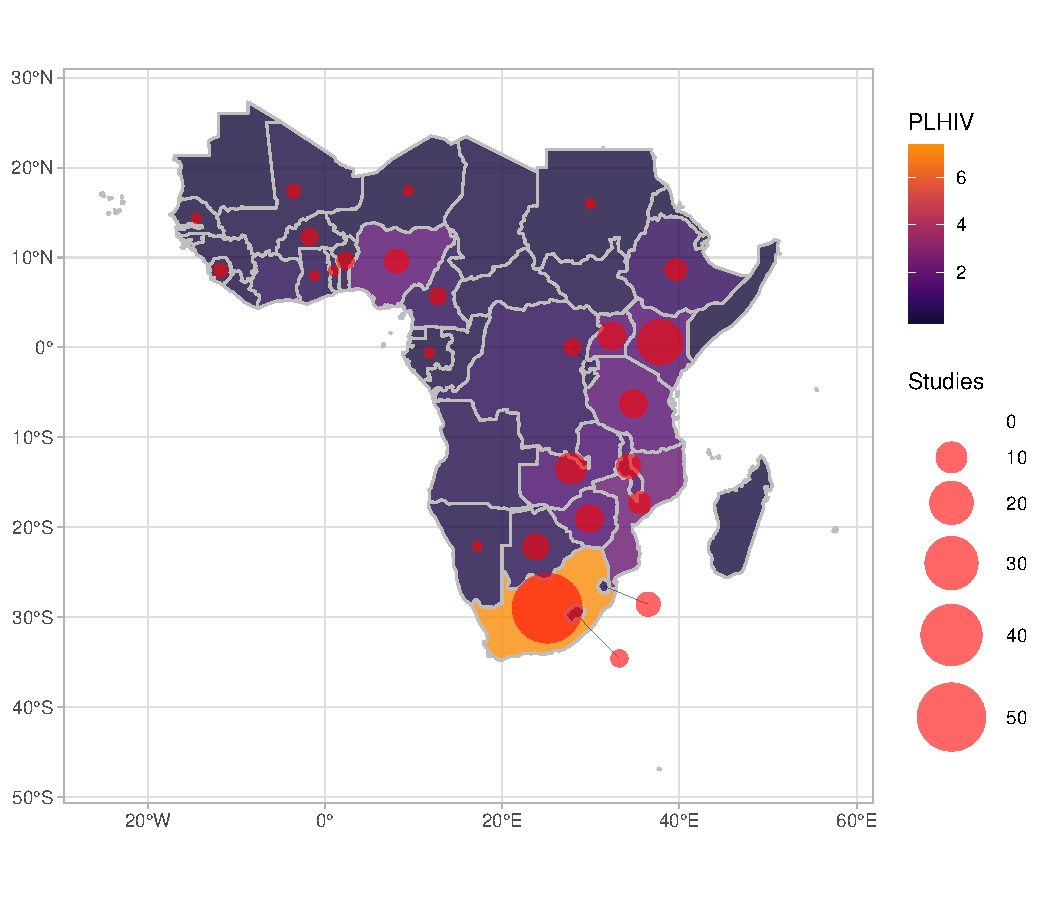
\includegraphics[width=0.8\textwidth]{map}
  \caption{Map showing number of studies (of 94 total)
    applying HIV transmission modelling in each country vs
    the number of people living with HIV (PLHIV, millions)}
  \label{fig:map}
\end{figure}
\clearpage % TEMP
% ==============================================================================
\subsection{Risk Heterogeneity}\label{aa:res:risk}
% ------------------------------------------------------------------------------
\subsubsection{Distributions}
The following figures illustrate the distributions (number of studies)
of various parameter values and modelling assumptions related to
factors of heterogeneity and intervention contexts.
\par
\foreach \var/\title in \plotlistdist{
  \begin{minipage}[t][.33\textheight][t]{0.48\linewidth}
    \includegraphics[width=0.95\textwidth]{{d.\var}.pdf}
    \captionof{figure}{\title}
    \label{fig:\var}
  \end{minipage}\hspace{0.04\linewidth}}
\clearpage
% ==============================================================================
\subsection{ART Prevention Impact}\label{aa:res:api}
The following figures illustrate the projected ART prevention impact (Dataset~B),
stratified by various factors of heterogeneity and intervention contexts (colours).
Left panels show the relative reduction in HIV incidence rate;
right panels show the relative reduction in cumulative new HIV infections;
both as compared to a base-case scenario reflecting status quo.
If any study included multiple scenarios of ART scale-up,
then each scenario was included separately;
if any scenario reported multiple time horizons,
each time horizon was included separately.
The number of studies (scenarios) reporting
incidence reduction, cumulative infections averted, both, or either was:
\x{n/n.a.api.inc}~(\x{n/n.s.api.inc}),
\x{n/n.a.api.chi}~(\x{n/n.s.api.chi}),
\x{n/n.a.api.both}~(\x{n/n.s.api.both}), and
\x{n/n.a.api}~(\x{n/n.s.api}), respectively.
If any factor could not be quantified due to missing data or varying values,
it was omitted from that plot.
In box plots, the numbers of unique scenario time-horizons
contributing to each box are given above it.
\begin{figure}[H]
  \begin{subfigure}{0.5\linewidth}
     \includegraphics[width=\linewidth]{{inc.s.Risk.both}.pdf}
    \caption{Reduction in HIV incidence (\%)}
  \end{subfigure}%
  \begin{subfigure}{0.5\linewidth}
     \includegraphics[width=\linewidth]{{chi.s.Risk.both}.pdf}
    \caption{Cumulative HIV infections averted (\%)}
  \end{subfigure}
  \caption{Projected ART prevention benefits,
    stratified by factors of risk heterogeneity: whether models considered
    differences in sexual activity, key populations, and
    ART cascade prioritized to key populations
    (subset of studies reporting both outcomes)}
  \label{fig:api:both}
\end{figure}
\foreach \var/\title in \plotlistapi{
  \begin{figure}[H]
    \begin{subfigure}{0.5\linewidth}
      \includegraphics[width=\linewidth]{{inc.\var}.pdf}
    \end{subfigure}%
    \begin{subfigure}{0.5\linewidth}
      \includegraphics[width=\linewidth]{{chi.\var}.pdf}
    \end{subfigure}
    \caption{\title}
    \label{fig:api:\var}
  \end{figure}
}
\begin{figure}[H]
  \centering
  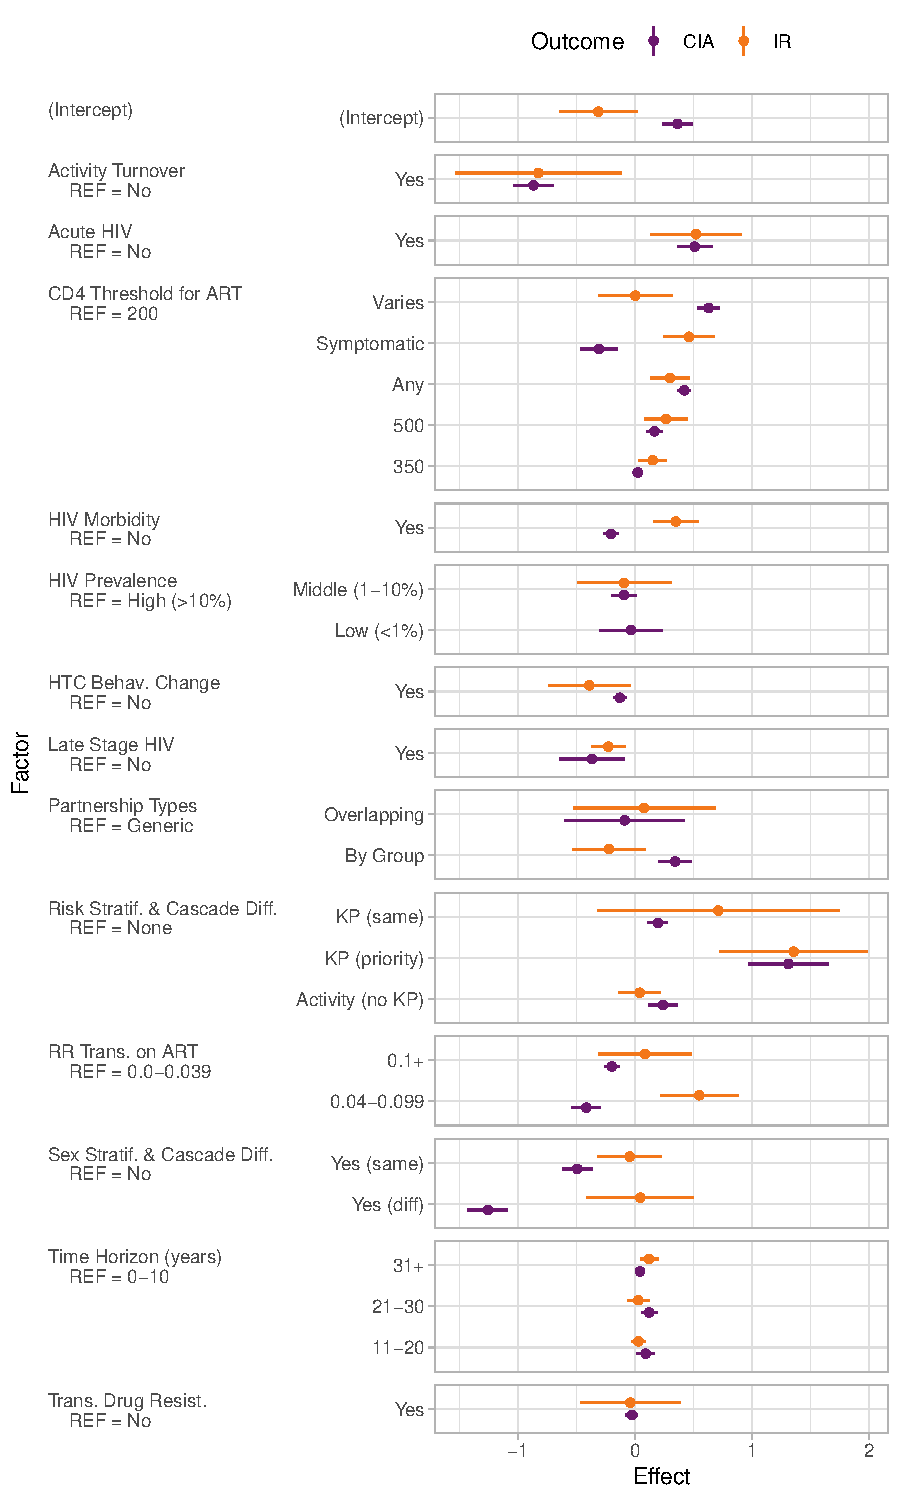
\includegraphics[width=0.75\linewidth]{effects}
  \caption{Effect estimates for factors of heterogeneity on
    incidence reduction (\%, IR) and cumulative infections averted (\%, CHI)
    from linear multivariate regression with generalized estimating equations.}
  \label{fig:effects}
  \floatfoot{
    Numerical results given in Table~\ref{tab:api}.
    RR: relative risk;
    HTC: HIV testing and counselling;
    KP: key populations.
    priority: modelled ART cascade transitions were faster in KP vs overall due to prioritized programs;
    same: cascade transitions were assumed the same in KP as overall.
    Factor definitions are given in Appendix~\ref{a:defs}.
  }
\end{figure}
%%%%%%%%%%%%%%%%%%%%%%%%%%%%%%%%%%%%%%%%%%%%%%%%%%%%%%%%%%%%%%%%%%%%%%%%%%%%%%%%
\end{document}
%%%%%%%%%%%%%%%%%%%%%%%%%%%%%%%%%%%%%%%%%%%%%%%%%%%%%%%%%%%%%%%%%%%%%%%%%%%%%%%%
